Testing concurrent programs cannot be done with conventional
techniques.  The nondeterminism of scheduling means that a test may
produce different results in different executions.  In this chapter we
give an introduction to concurrency testing through \emph{controlled
  scheduling}, which addresses this problem.  Controlled scheduling is
the foundation upon which we build our work.  We first give a
high-level overview~\sref{sct-fundamentals}, then discuss specific
implementation approaches, both complete~\sref{sct-dpor} and
incomplete~\sref{sct-bounding}.  We then discuss two tools for
concurrency testing in functional languages~\sref{sct-functional}.

This chapter is presented in a very different style to
\Cref{chp:concurrent_haskell}.  We are now discussing ideas and
approaches, rather than the specifics of particular programming
languages.

\section{Controlled Scheduling}
\label{sec:sct-fundamentals}

With a controlled scheduling technique, execution of a program is
serialised and the controlling scheduler drives the program.  Program
schedules are either explored
\emph{systematically}\cite{coons2013,flanagan2005,musuvathi2008,musuvathi2007}
(often called `systematic concurrency testing' or `SCT') or
randomly\cite{burckhardt2010,thomson2016}.  Non-controlled methods do
not provide their own scheduler, and instead use delays and priorities
to affect execution\cite{yu2012}.  Controlled scheduling techniques
are attractive because of their ability to record and replay program
executions.

Controlled scheduling can be implemented by overriding the concurrency
primitives of the language\cite{walker2015}; by instrumenting the
source program\cite{claessen2009}; or by instrumenting the compiled
program\cite{musuvathi2006,yu2012}.  Systematic techniques may be
\emph{complete}: able to find all distinct results of a program.
Random techniques typically cannot ensure that all distinct results
are found, cannot be complete, and are usually run for some
predetermined number of program executions.

Typically we assume that all possible executions are
\emph{terminating}: leading to successful completion or a failure
state such as deadlock.  Another common assumption is that the number
of possible executions is \emph{finite}: forbidding finite but
arbitrarily long executions, as can be created with constructs such as
spinlocks\cite{siberschatz1993}.  We can sacrifice completeness to do
away with these assumptions, as we shall see in
\Cref{sec:sct-bounding}.

\section{Dynamic Partial-order Reduction}
\label{sec:sct-dpor}

Dynamic partial-order reduction (DPOR)\cite{flanagan2005,godefroid1996} is a
\emph{complete} approach to SCT\@.  It is based on the insight that, when
constructing schedules, we only need to consider different orderings of a pair
of actions if the order in which they are performed could affect the
result of the program.  We call this relation between actions
the \emph{dependency relation}.

\begin{displayquote}
  \textbf{Definition} (Dependency Relation\cite{flanagan2005})

  \noindent
  Let $\mathcal T$ be the set of transitions in a concurrent system.  A binary,
  reflexive, and symmetric relation $\mathcal D \subseteq \mathcal
  T \times \mathcal T$ is a valid dependency relation iff, for all $t_{1},
  t_{2} \in \mathcal T$, $(t_{1}, t_{2}) \notin \mathcal D$ ($t_{1}$ and $t_{2}$
  are independent) the following properties hold for all program states $s$:

  \begin{enumerate}
  \item if $t_{1}$ is enabled in $s$ and $s \xrightarrow{t_{1}} s'$, then
    $t_{2}$ is enabled in $s$ iff $t_{2}$ is enabled in $s'$; and

  \item if $t_{1}$ and $t_{2}$ are enabled in $s$, then there is a unique state
    $s'$ such that $s \xrightarrow{t_{1}t_{2}} s'$ and
    $s \xrightarrow{t_{2}t_{1}} s'$.
    \hfill$\blacksquare$
  \end{enumerate}
\end{displayquote}

In other words, independent transitions cannot enable (unblock) or
disable (block) each other, and enabled independent transitions
commute.  When implementing DPOR, we typically identify a sufficient
condition for dependency, rather than work with this relational
definition directly.

Typically, the presentation of algorithms assumes a simple core
concurrent language of just reads and writes.  This gives rise to a
relation such as: $x$ and $y$ are dependent if and only if they are
actions in the same thread, or they are actions involving the same
variable where at least one is a write.  We can express this
dependency relation like so:

\begin{align*}
  x \dependent y \iff& \mathrm{thread\_id}(x) = \mathrm{thread\_id}(y)~\lor\\
    &\left(\mathrm{variable}(x) = \mathrm{variable}(y)
     \land \left(\mathrm{is\_write}(x) \lor \mathrm{is\_write}(y)\right)\right)
\end{align*}

The notation $x \dependent y$ is read as ``$x$ and $y$ are
dependent.''  This choice of notation would suggest $\leftrightarrow$
for independence, but that doesn't seem to be in common use.

\Cref{fig:dpor} shows an example of DPOR in action.  There are two
threads: thread 1 performs reads from two variables \verb|x| and
\verb|y|, and thread 2 writes to \verb|y|.  As \verb|read x| is
independent from \verb|write y|, DPOR prunes one ordering of those
actions.

\begin{figure}
  \centering
  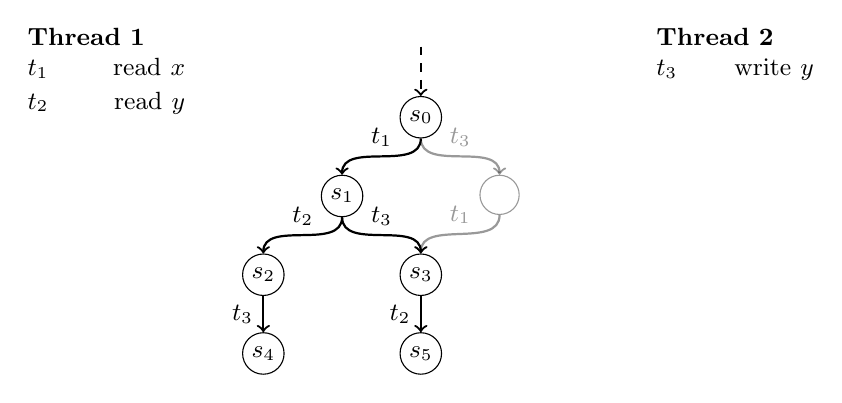
\begin{tikzpicture}[ball/.style = {circle, draw, align=center, anchor=north, inner sep=0, text width=0.5cm}]
    \node[ball]              (A) at (0,0)   {\small $s_0$};
    \node[ball]              (B) at (-1,-1) {\small $s_1$};
    \node[ball]              (C) at (-2,-2) {\small $s_2$};
    \node[ball]              (D) at (-2,-3) {\small $s_4$};
    \node[ball, opacity=0.4] (E) at (1,-1) {};
    \node[ball]              (F) at (0,-2) {\small $s_3$};
    \node[ball]              (G) at (0,-3) {\small $s_5$};

    \node (init) at (0,0.75) {};
    \draw[->, thick, draw, dashed] (init.south) to [out=270,in=90] (A.north);

    \draw[->, thick, draw]              (A.south) to [out=270,in=90] node[midway,above] {\small $t_1$} (B.north);
    \draw[->, thick, draw]              (B.south) to [out=270,in=90] node[midway,above] {\small $t_2$} (C.north);
    \draw[->, thick, draw]              (C.south) to [out=270,in=90] node[midway,left]  {\small $t_3$} (D.north);
    \draw[->, thick, draw, opacity=0.4] (A.south) to [out=270,in=90] node[midway,above] {\small $t_3$} (E.north);
    \draw[->, thick, draw]              (B.south) to [out=270,in=90] node[midway,above] {\small $t_3$} (F.north);
    \draw[->, thick, draw, opacity=0.4] (E.south) to [out=270,in=90] node[midway,above] {\small $t_1$} (F.north);
    \draw[->, thick, draw]              (F.south) to [out=270,in=90] node[midway,left]  {\small $t_2$} (G.north);

    \node[anchor=west,text width=2cm, text depth=1.5cm, inner sep=0] (note1) at (-5,0) {
      \small
      \textbf{Thread 1}\\
      $t_1$ \hfill read $x$\\
      $t_2$ \hfill read $y$
    };

    \node[anchor=east,text width=2cm, text depth=1.5cm, inner sep=0] (note2) at (5,0) {
      \small
      \textbf{Thread 2}\\
      $t_3$ \hfill write $y$\\
    };
  \end{tikzpicture}
  \caption[How DPOR prunes the space of schedules.]{How DPOR prunes the space of schedules.  Transition $t_3$ is pruned in state $s_0$ because it is independent with transition $t_1$.  Adapted from \cite{coons2013}.}\label{fig:dpor}
\end{figure}

Our dependency relation for Haskell~\sref{dejafu-testing} is rather
more complex, as there are more actions than just reads and writes.
We express it as a few general conditions over different sorts of
reads and writes, with a collection of special cases for software
transactional memory and exceptions.  Additionally, a Haskell program
terminates when the main thread terminates, which complicates matters
further.  A na\"{\i}ve implementation of this, imposing a dependency
between the final action of the main thread and everything else, leads
to too many executions being tried to be of practical use.  We discuss
these issues further in \Cref{sec:dejafu-testing}.

\subsection{Total and Partial Orders}

Characterising the execution of a concurrent program by the ordering
of its dependent actions gives us a \emph{partial} order over the
actions in the entire program.  An execution trace is just one
possible \emph{total} order, a refinement of the constraining partial
order.  We call the equivalence class of total orders corresponding to
the same partial order a \emph{Mazurkiewicz
  trace}\cite{mazurkiewicz1986}.  The goal of partial-order reduction,
then, is to only try one total order for each distinct Mazurkiewicz
trace, by intelligently making scheduling decisions to permute the
order of dependent actions.

DPOR is so called because it gathers information about the
dependencies between threads dynamically at run-time, to avoid the
imprecision of static analyses\cite{flanagan2005}.  It works by
executing the program until completion, making arbitrary choices to
resolve scheduling nondeterminism, dynamically collecting information
about how threads have behaved during this specific execution.  This
execution trace is then examined to identify places where alternative
scheduling decisions need to be explored because they might lead to
other executions which correspond to a different partial-order.  The
algorithm repeats until all backtracking points have been explored and
no new ones are found.  So it only works if all executions are
terminating and the number of distinct executions is finite.  DPOR is
complete.  When it terminates, all distinct states of the program will
have been explored.

\subsection{Relaxed Memory Models}

In the name of performance, modern processors often implement memory
models that are weaker than sequential consistency\cite{lamport1979}
by using optimisations such as speculative execution, buffering, and
caching.  Unlike sequential consistency, where a concurrent program
behaves as a simple interleaving of atomic thread actions, relaxed
memory models can be more complex, making program analysis and
debugging difficult.  For example, under Total Store Order (TSO),
which x86 processors use\cite{owens2009}, reads and writes in the same
thread to different memory locations may be re-ordered.  Under Partial
Store Order (PSO), a relaxation of TSO\cite{sparc}, two writes in the
same thread, but to different memory locations, may also be reordered.

A simple buffering technique can be used model the nondeterminism of
these unsynchronised operations under TSO and PSO\cite{zhang2015}:

\begin{itemize}
\item Under TSO, each thread has a queue of buffered writes.
\item Under PSO, each thread has a queue of buffered writes for each shared
variable.
\end{itemize}

When reading, a thread reads its most recently buffered write.  If a
thread has no writes buffered to that variable, it reads the most
recently committed value.  A buffered write is only visible to the
thread which made it.  Buffered writes are committed
nondeterministically.  To model this, we can introduce one additional
\emph{phantom thread} for each nonempty buffer.  When scheduled, a
phantom thread commits the oldest write from its buffer.

SCT techniques assume that there is only one source of nondeterminism:
the scheduler.  If a second source is added, such as when writes are
committed, it is difficult to adapt existing algorithms directly.
But, by using phantom threads, the two sources of nondeterminism are
unified, and existing algorithms just work\cite{zhang2015}.

\subsection{Maximal Causality Reduction}

\emph{Maximal causality reduction} (MCR)\cite{huang2015,huang2017} is
an alternative to DPOR which explores a provably minimal number of
executions.  Consider these three threads:

\begin{center}
\verb|p: write x       q: write x      r: read x|
\end{center}

All pairs of actions are dependent, and so DPOR would explore all six
interleavings: \texttt{pqr}, \texttt{prq}, \texttt{qpr}, \texttt{qrp},
\texttt{rpq}, \texttt{rqp}.  However, if we consider which write is
read by thread \texttt{r}, many of these interleavings are equivalent.
For example, \texttt{pqr} results in the same value being read as
\texttt{qrp}.  In fact we only need to explore half of the
interleavings to find all the distinct values read.  Program execution
is driven by what values different threads read.  An unread write
changes nothing.  So ideally we would only try a schedule if it leads
to at least one distinct value being read.

The MCR algorithm is similar in outline to DPOR\@.  It performs an
execution, resolving scheduling nondeterminism arbitrarily, and
gathers a trace including information about the thread communication.
It then uses this trace to compute new schedule prefixes.  The
difference from DPOR is that these schedule prefixes ensure that at
least one read produces a previously unseen value.  MCR uses the trace
to compute a model of program behaviour as a set of quantifier-free
first-order logical formulae.  These formulae can then be augmented
with a state-change requirement and given to an SMT
solver\cite{demoura2011}, such as z3\cite{demoura2008}, to produce new
schedule prefixes.  When executed on benchmark programs, MCR
outperforms DPOR by orders of magnitude\cite{huang2017}.

MCR imposes one additional restriction which makes it tricky for
Haskell.  MCR requires a concurrency model to be \emph{locally
  deterministic}\cite{huang2015}.  Only the previous actions of a
thread and values read from shared variables, and not actions of other
threads, determine the next action of the thread.  This is not the
case for Haskell, where one thread may kill another by throwing an
exception to it.  However, it may be possible to encode Haskell
exceptions in an MCR-friendly way by giving each thread an exception
variable, and inserting reads to this variable before every normal
action.  Even after this modification some difficulty remains, as even
blocked threads may be interrupted by exceptions in Haskell.

Like DPOR, MCR can be extended to support the relaxed memory models TSO and
PSO\cite{huang2016}.

\section{Schedule Bounding}
\label{sec:sct-bounding}

Schedule bounding\cite{emmi2011,musuvathi2008,musuvathi2007} is an
\emph{incomplete} approach to concurrency testing.  A \emph{bound function} is
defined which associates a sequence of scheduling decisions with some value of a
type that has a total order, such as the integers.  This function is
monotonically increasing: if some sequence has an associated value of $n$, all
its prefixes will have an associated value of at most $n$.  This value $n$ is
limited by some pre-determined bound.  Testing proceeds by executing all
schedules within the bound.

A common schedule bounding approach is \emph{pre-emption
  bounding}\cite{musuvathi2007}, which limits the number of
pre-emptive context switches.  Empirical evidence shows that small
bounds, and small numbers of threads, are effective for finding many
real-world bugs\cite{thomson2014}.

Another common approach is \emph{fair bounding}\cite{musuvathi2008},
which bounds the difference between how many times any two threads may
explicitly yield.  This prevents infinitely long executions when using
constructs such as spinlocks, which loop until some condition holds,
yielding on every iteration it does not.

Bound functions can be combined, where a sequence of scheduling
decisions is outside the combined bound if it is outside either of the
constituent bounds.

Schedule bounding traditionally refers to trying only those schedules
with a bound value equal to a fixed parameter.  A variant is
\emph{iterative} bounding, where the parameter is gradually
increased\cite{musuvathi2007}.  Another variant is where an
inequality, rather than an equality, is used.  This variant explores
the same schedules as iterative bounding, but doesn't impose the same
ordering.  In practice, `schedule bounding' typically refers to this
third type.

\subsection{Integration with DPOR}

Schedule bounding can be combined with DPOR to produce a technique
which is complete within its bound.  The na\"{\i}ve way to integrate
these techniques would be to first use partial-order techniques to
prune the search space, and then to additionally filter things out
with schedule bounding.  However, this is unsound.  As
\Cref{fig:bpor_unsound} shows, this approach misses parts of the
search space reachable within the bound.  This is because the
introduction of the bound creates new dependencies between actions,
which cannot be determined \emph{a priori}\cite{coons2013}.

\begin{figure}
  \centering
  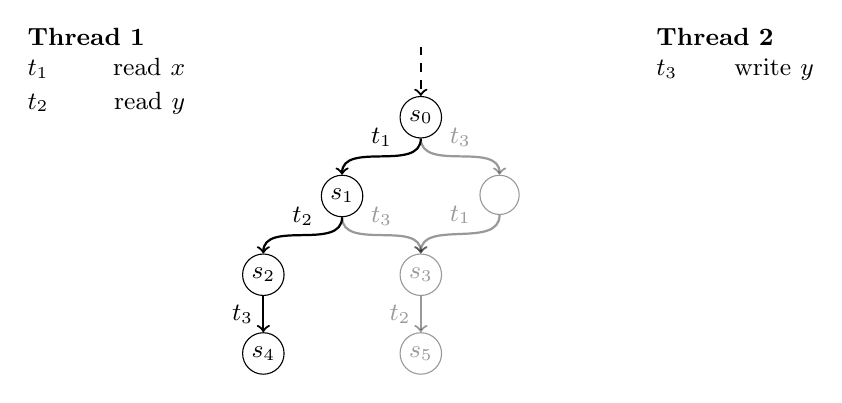
\begin{tikzpicture}[ball/.style = {circle, draw, align=center, anchor=north, inner sep=0, text width=0.5cm}]
    \node[ball]              (A) at (0,0)   {\small $s_0$};
    \node[ball]              (B) at (-1,-1) {\small $s_1$};
    \node[ball]              (C) at (-2,-2) {\small $s_2$};
    \node[ball]              (D) at (-2,-3) {\small $s_4$};
    \node[ball, opacity=0.4] (E) at (1,-1) {};
    \node[ball, opacity=0.4] (F) at (0,-2) {\small $s_3$};
    \node[ball, opacity=0.4] (G) at (0,-3) {\small $s_5$};

    \node (init) at (0,0.75) {};
    \draw[->, thick, draw, dashed] (init.south) to [out=270,in=90] (A.north);

    \draw[->, thick, draw]              (A.south) to [out=270,in=90] node[midway,above] {\small $t_1$} (B.north);
    \draw[->, thick, draw]              (B.south) to [out=270,in=90] node[midway,above] {\small $t_2$} (C.north);
    \draw[->, thick, draw]              (C.south) to [out=270,in=90] node[midway,left]  {\small $t_3$} (D.north);
    \draw[->, thick, draw, opacity=0.4] (A.south) to [out=270,in=90] node[midway,above] {\small $t_3$} (E.north);
    \draw[->, thick, draw, opacity=0.4] (B.south) to [out=270,in=90] node[midway,above] {\small $t_3$} (F.north);
    \draw[->, thick, draw, opacity=0.4] (E.south) to [out=270,in=90] node[midway,above] {\small $t_1$} (F.north);
    \draw[->, thick, draw, opacity=0.4] (F.south) to [out=270,in=90] node[midway,left]  {\small $t_2$} (G.north);

    \node[anchor=west,text width=2cm, text depth=1.5cm, inner sep=0] (note1) at (-5,0) {
      \small
      \textbf{Thread 1}\\
      $t_1$ \hfill read $x$\\
      $t_2$ \hfill read $y$
    };

    \node[anchor=east,text width=2cm, text depth=1.5cm, inner sep=0] (note2) at (5,0) {
      \small
      \textbf{Thread 2}\\
      $t_3$ \hfill write $y$\\
    };
  \end{tikzpicture}
  \caption[The na\"{\i}ve, unsound, way to combine DPOR with schedule bounding.]{The na\"{\i}ve, unsound, way to combine DPOR with schedule bounding.  Transition $t_3$ is pruned in state $s_0$ because it is independent with transition $t_1$.  Transition $t_3$ may be pruned in state $s_1$ because it causes a pre-emption.  If it is, the unique states $s_3$ and $s_5$ are never reached, despite being reachable within the bound from state $s_0$.  Adapted from \cite{coons2013}.}\label{fig:bpor_unsound}
\end{figure}

The solution is to add \emph{conservative} backtracking points to
account for the bound in addition to any normal backtracking points
that are identified.  Where to insert these depends on the bound
function.  In the case of pre-emption bounding, it is sufficient to
try all possibilities at the last context switch before a normal
backtracking point\cite{coons2013}.  This is because context switches
influence the number of pre-emptions needed to reach a given program
state, depending on which thread gets scheduled.  So in
\Cref{fig:bpor_unsound}, the transition $t_3$ in state $s_0$ would be
added as a conservative backtracking point, undoing the work of DPOR
in that case.  In practice the addition of backtracking points in this
way tends not to greatly increase the search space\cite{coons2013}.

\section{In Functional Languages}
\label{sec:sct-functional}

\paragraph{In Erlang}
\textsc{Pulse}\cite{claessen2009} is a controlled scheduler for Erlang
programs which implements co-operative multi-tasking.  An
instrumentation process automatically modifies existing programs to
call out to this scheduler.  \textsc{Pulse} works by only allowing one
of the concurrent processes to operate at a time, and makes scheduling
decisions around effectful actions: such as a process receiving a
message.  It also allows interaction with uninstrumented functions,
which are treated as atomic, allowing tested subsystems to be composed
without exploring interleavings within the subsystem.  \textsc{Pulse}
scheduling decisions are made randomly, using a given seed, and a
complete execution trace is returned.  The trace can be rendered into
a graphical form showing the interactions between threads to aid
debugging.  The authors report that the graphical traces often suggest
potential race conditions not otherwise apparent to a human reader.

\emph{Procrastination}\cite{sen2008} is used to improve detection of
bugs.  First \textsc{Pulse} is used to produce an execution trace,
which is then examined to find pairs of dependent actions, as in DPOR.
Then, for each pair, execution proceeds with a random scheduler.  When
one of the actions in an identified dependent pair is encountered, the
thread is instead paused until another thread is about to resolve the
other action.  The race is then randomly resolved and execution
continues.  Rather than exploring all partial orders, this approach is
a probabilistic one, but it is guaranteed to explore only
\emph{racing} partial orders.  This approach has an advantage in
programs which have many non-racy partial orders, where randomly
choosing between them does not reliably produce a bug.  The authors
report that improvements can result in new bugs being found, although
in the cases where the procrastination was not necessary to find the
bug, performance degrades\cite{arts2011} as one test with
procrastination corresponds to multiple executions with different
schedules.

\paragraph{In Haskell}
The Concurrent Haskell Debugger (CHD)\cite{bottcher2002} is a
GUI-based controlled scheduler for Haskell programs.  Like
\textsc{Pulse}, CHD works by inserting blocking communication
operations around concurrency actions to call out to the controlling
scheduler.  Unlike \textsc{Pulse}, this process is not quite
automatic.  The programmer must import the concurrency module provided
by the CHD library, rather than the standard library.  CHD does not
implement its own scheduler.  Rather, it presents a GUI to the user,
allowing them to drive execution by clicking representations of
threads.  Furthermore, it allows the user to specify cases which
should be automatically allowed to execute.  CHD does not function
with any GHC newer than version 5 (released between 2001 and 2003).

\vfill\pagebreak
\section{Summary}

Going forward, the reader should keep in mind:

\begin{itemize}
\item Controlled scheduling techniques use a user-level scheduler to
  drive the execution of concurrent program.  This can be done by
  overriding the concurrency primitives of the source language;
  instrumenting the program source code; or instrumenting the compiled
  program~\sref{sct-fundamentals}.

\item Systematic concurrency testing (SCT) is an umbrella term for a
  collection of techniques for exploring the behaviours of concurrent
  programs, through controlled scheduling~\sref{sct-fundamentals}.

\item Dynamic partial-order reduction (DPOR), which falls under the
  SCT umbrella, is a technique to discover all distinct states of a
  concurrent program.  DPOR takes advantage of mutually commuting
  operations to reduce space of schedules to explore~\sref{sct-dpor}.

\item Schedule bounding is a technique to reduce the space of
  schedules to explore by simply discarding any which exceed some
  chosen bound, such as the number of pre-emptive context switches.
  Schedule bounding will not, in general, find all distinct states of
  a concurrent program~\sref{sct-bounding}.
\end{itemize}

We revisit DPOR and schedule bounding in \Cref{chp:dejafu}, where we
discuss our tool for testing concurrent Haskell programs.  We revisit
controlled scheduling more generally in \Cref{chp:algorithms}, where
we propose a new scheduling algorithm for exposing concurrency bugs.
